\documentclass[../main.tex]{subfiles}

\begin{document}

Pierwszy widok prezentowany użytkownikowi na stronie to widok główny (rys. \ref{fig:instrukcja_uzytkowania:home}). Z widoku głównego niezalogowany użytkownik ma możliwość przeglądania najpopularniejszych filmów oraz ostatnich recenzji i komentarzy. 

\begin{figure}[htb]
	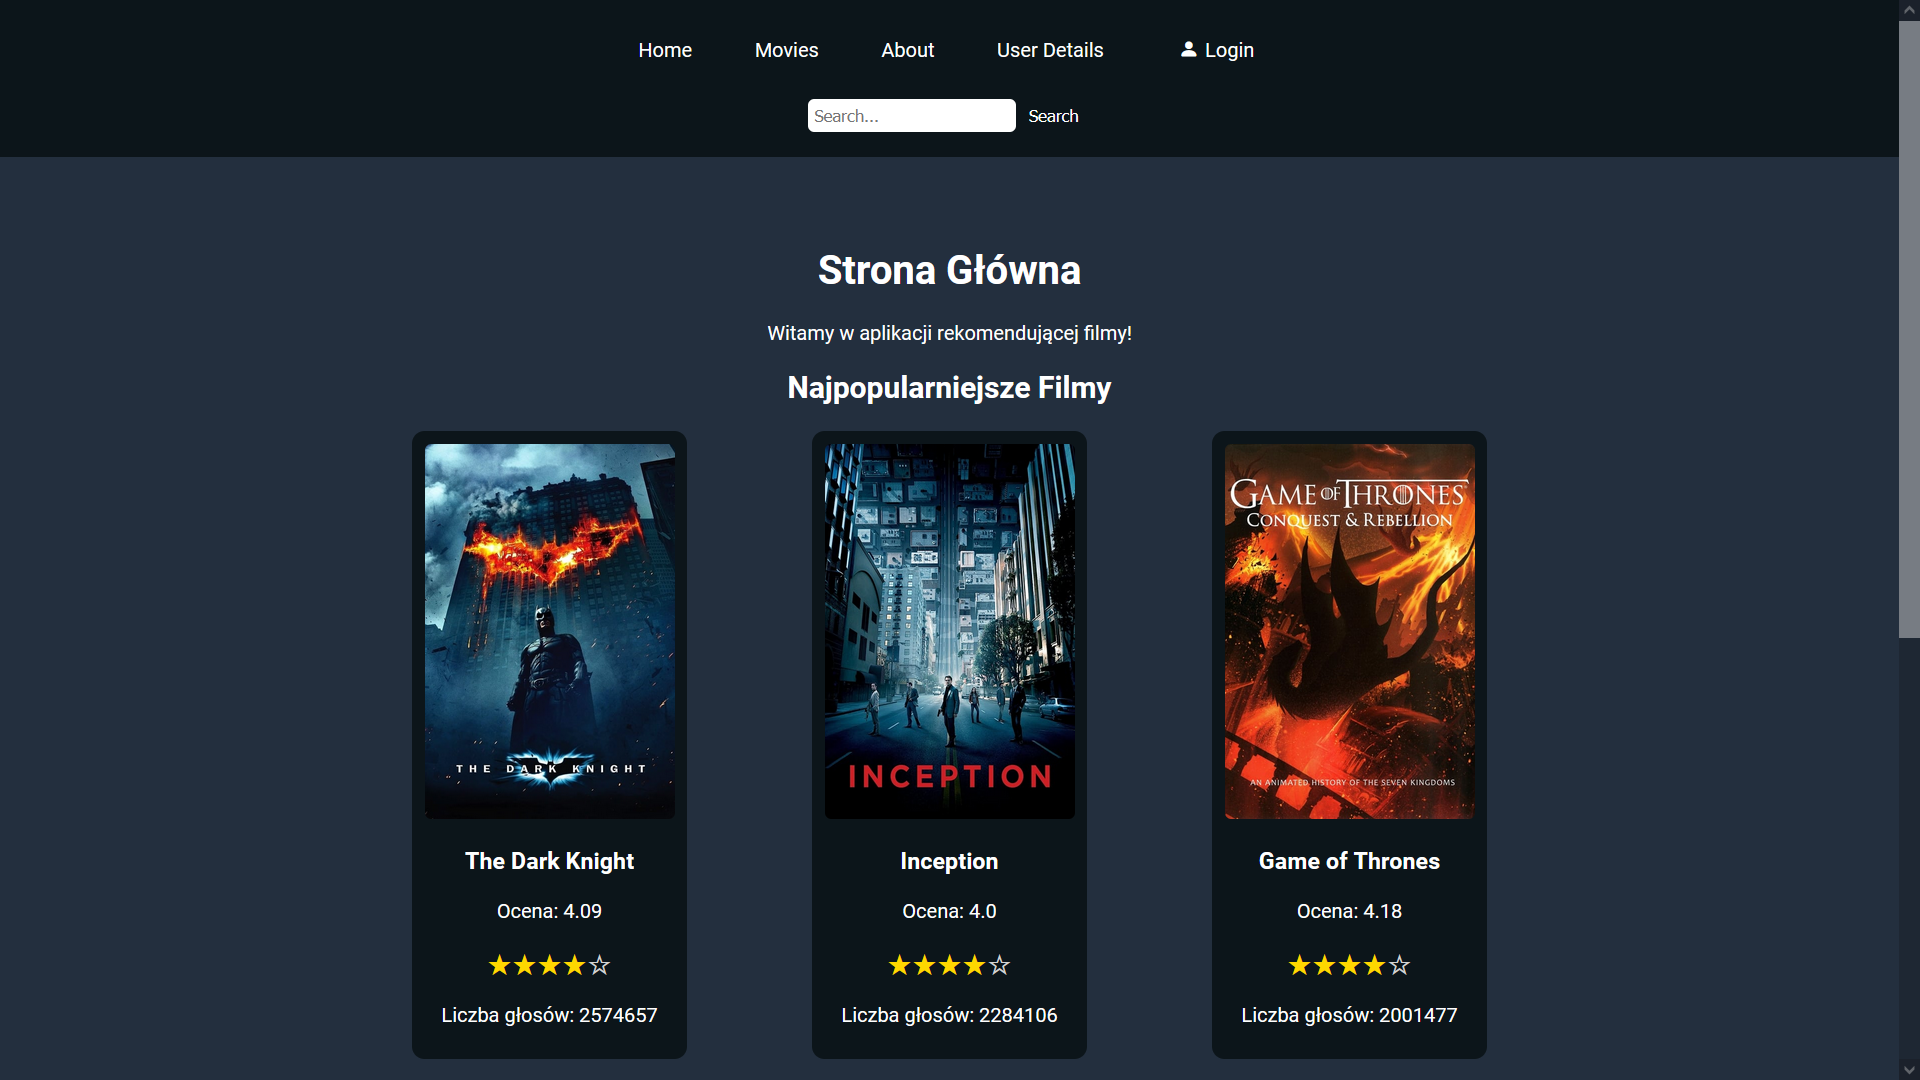
\includegraphics[width=\textwidth]{instrukcja_uzytkowania/home.png}
	\caption{Widok główny}
	\label{fig:instrukcja_uzytkowania:home}
\end{figure}

Na pasku nawigacji niezalogowany użytkownik ma wymienione 4 pozycje:
\begin{itemize}
	\item \textit{Home}: obecny widok (widok główny),
	\item \textit{Movies}: widok filmów,
	\item \textit{About}: widok informacji o stronie,
	\item \textit{User Details}: widok informacji o użytkowniku (dostępny tylko po zalogowaniu).
	\item \textit{Login}: widok logowania.
\end{itemize}

Pasek nawigacji pozostaje niezmienny przez wszystkie widoki.
Po przejściu do widoku \textit{Movies} (rys. \ref{fig:instrukcja_uzytkowania:movies}), użytkownikowi zostaje zaprezentowany pełen repertuar dostępnych na stronie filmów. Możliwe jest również wpisanie żądanej frazy w pasku wyszukiwania na górze, aby otrzymać pasujące filmy.

\begin{figure}[htb]
	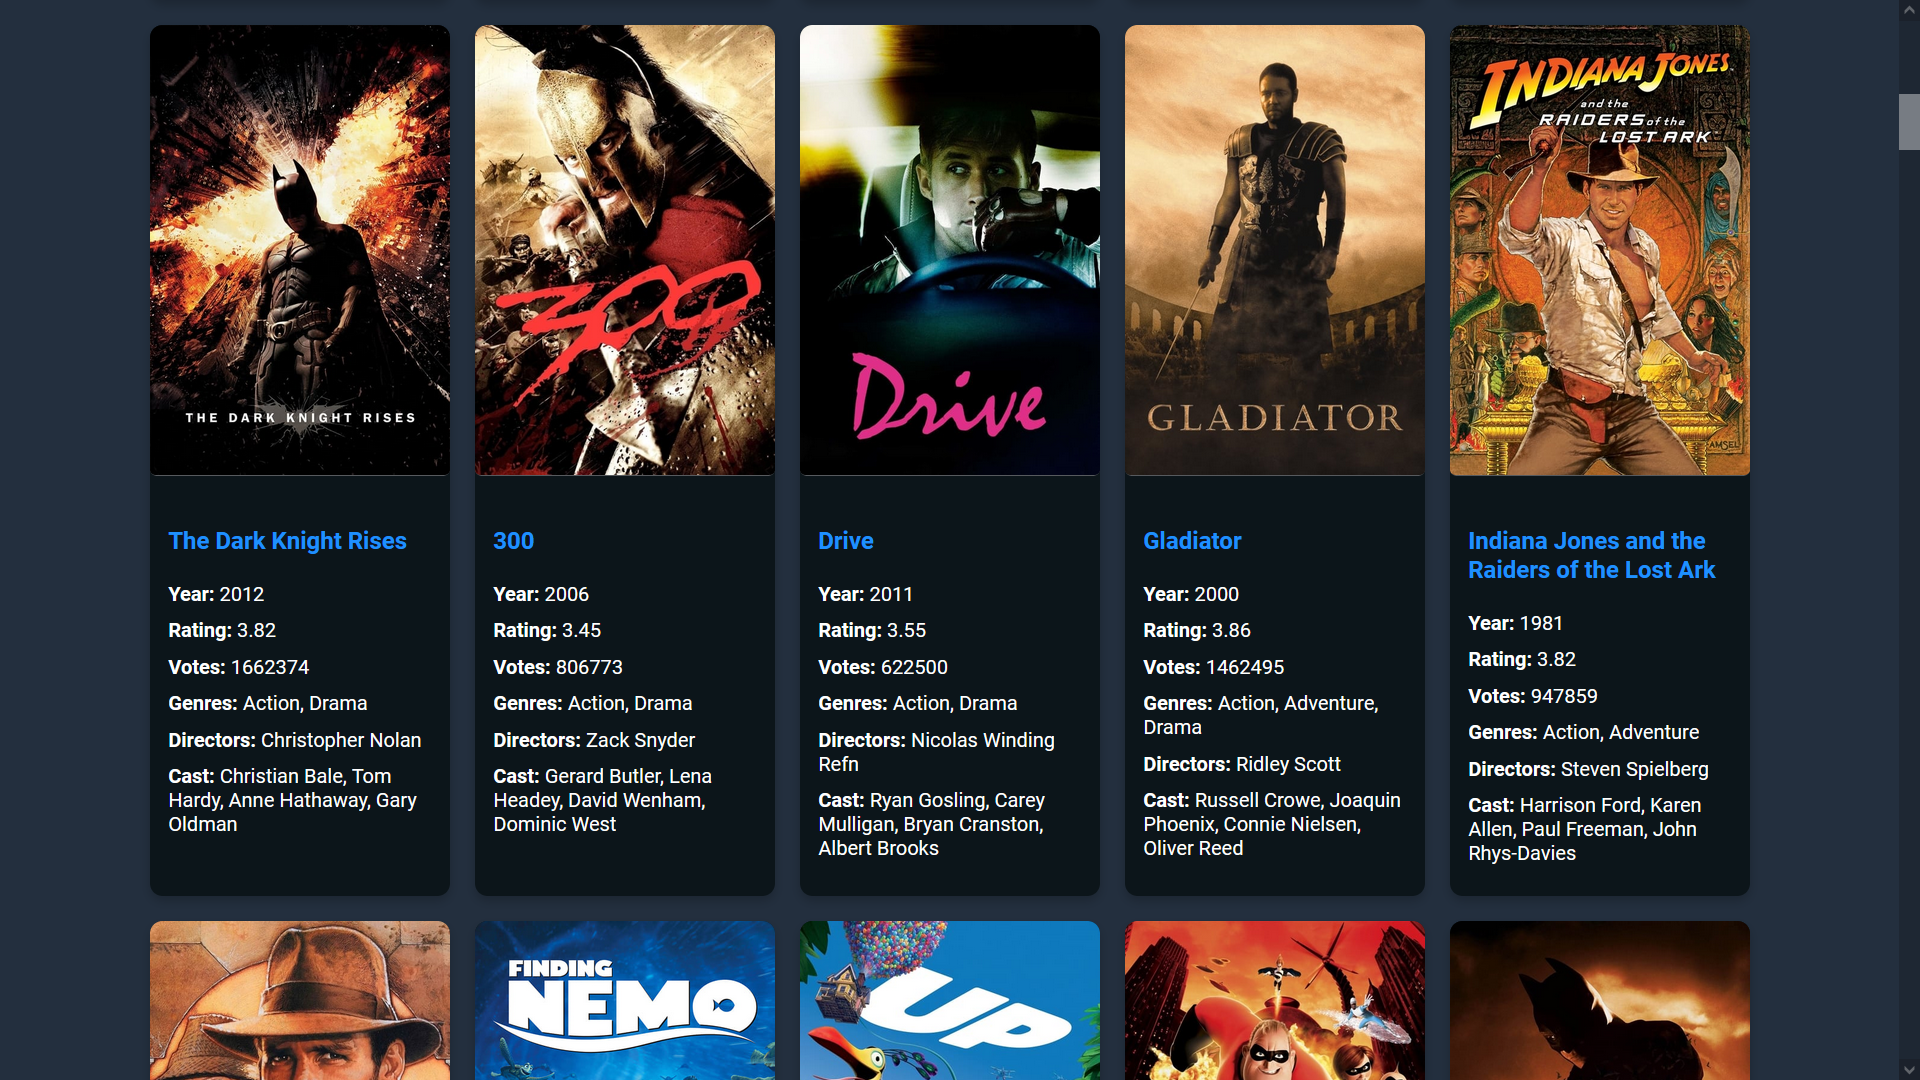
\includegraphics[width=\textwidth]{instrukcja_uzytkowania/movies.png}
	\caption{Widok filmów}
	\label{fig:instrukcja_uzytkowania:movies}
\end{figure}

Po kliknięciu karty filmu, użytkownik zostaje przekierowany do widoku filmu (rys. \ref{fig:instrukcja_uzytkowania:movie}). W nim znajduje się opis filmu, obsada, reżyser oraz pozostałe informacje o filmie. Po zjechaniu w dół strony można znaleźć sekcję recenzji filmu (rys. \ref{fig:instrukcja_uzytkowania:movie_reviews}). Znajdują się tam recenzje użytkowników na temat filmu. Zalogowany użytkownik ma w tym widoku możliwość wystawienia własnej opinii na temat filmu, bądź też skomentowania go.

\begin{figure}[htb]
	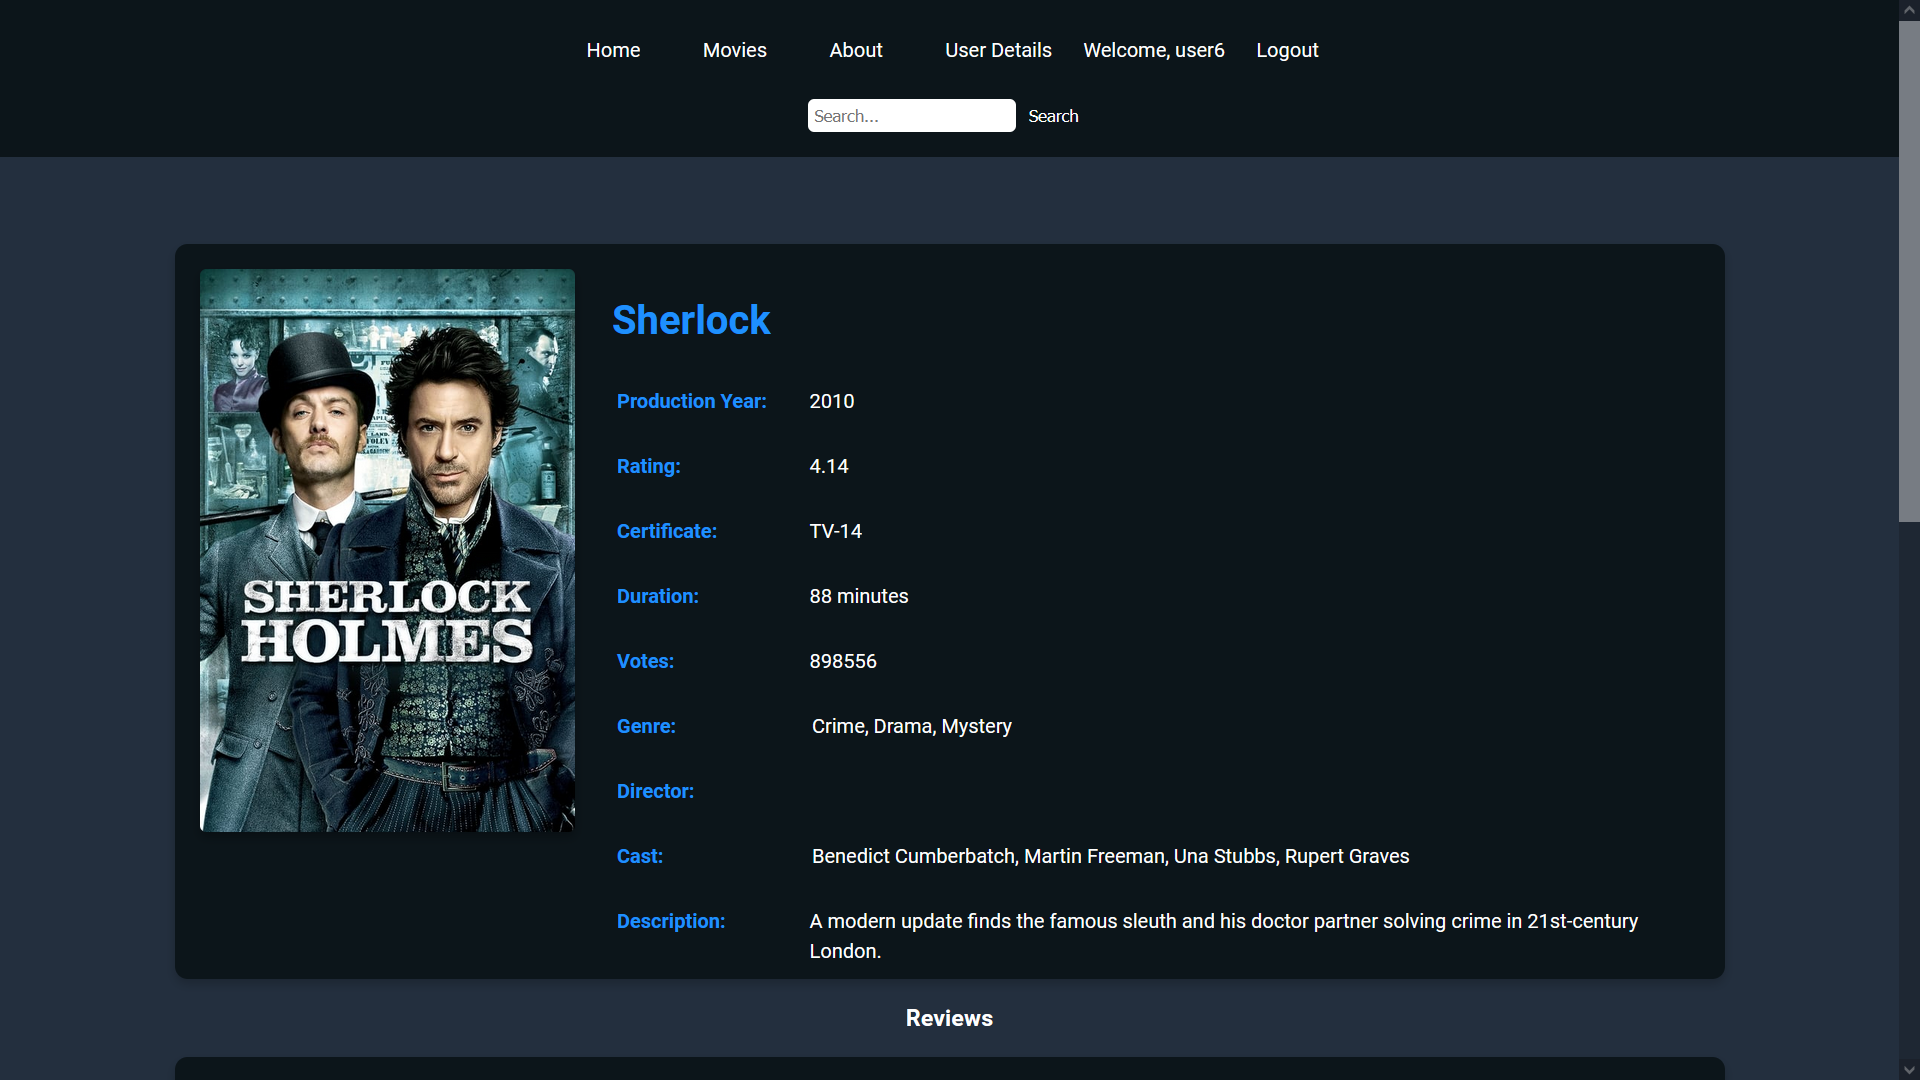
\includegraphics[width=\textwidth]{instrukcja_uzytkowania/movie.png}
	\caption{Widok filmu}
	\label{fig:instrukcja_uzytkowania:movie}
\end{figure}
\begin{figure}[htb]
	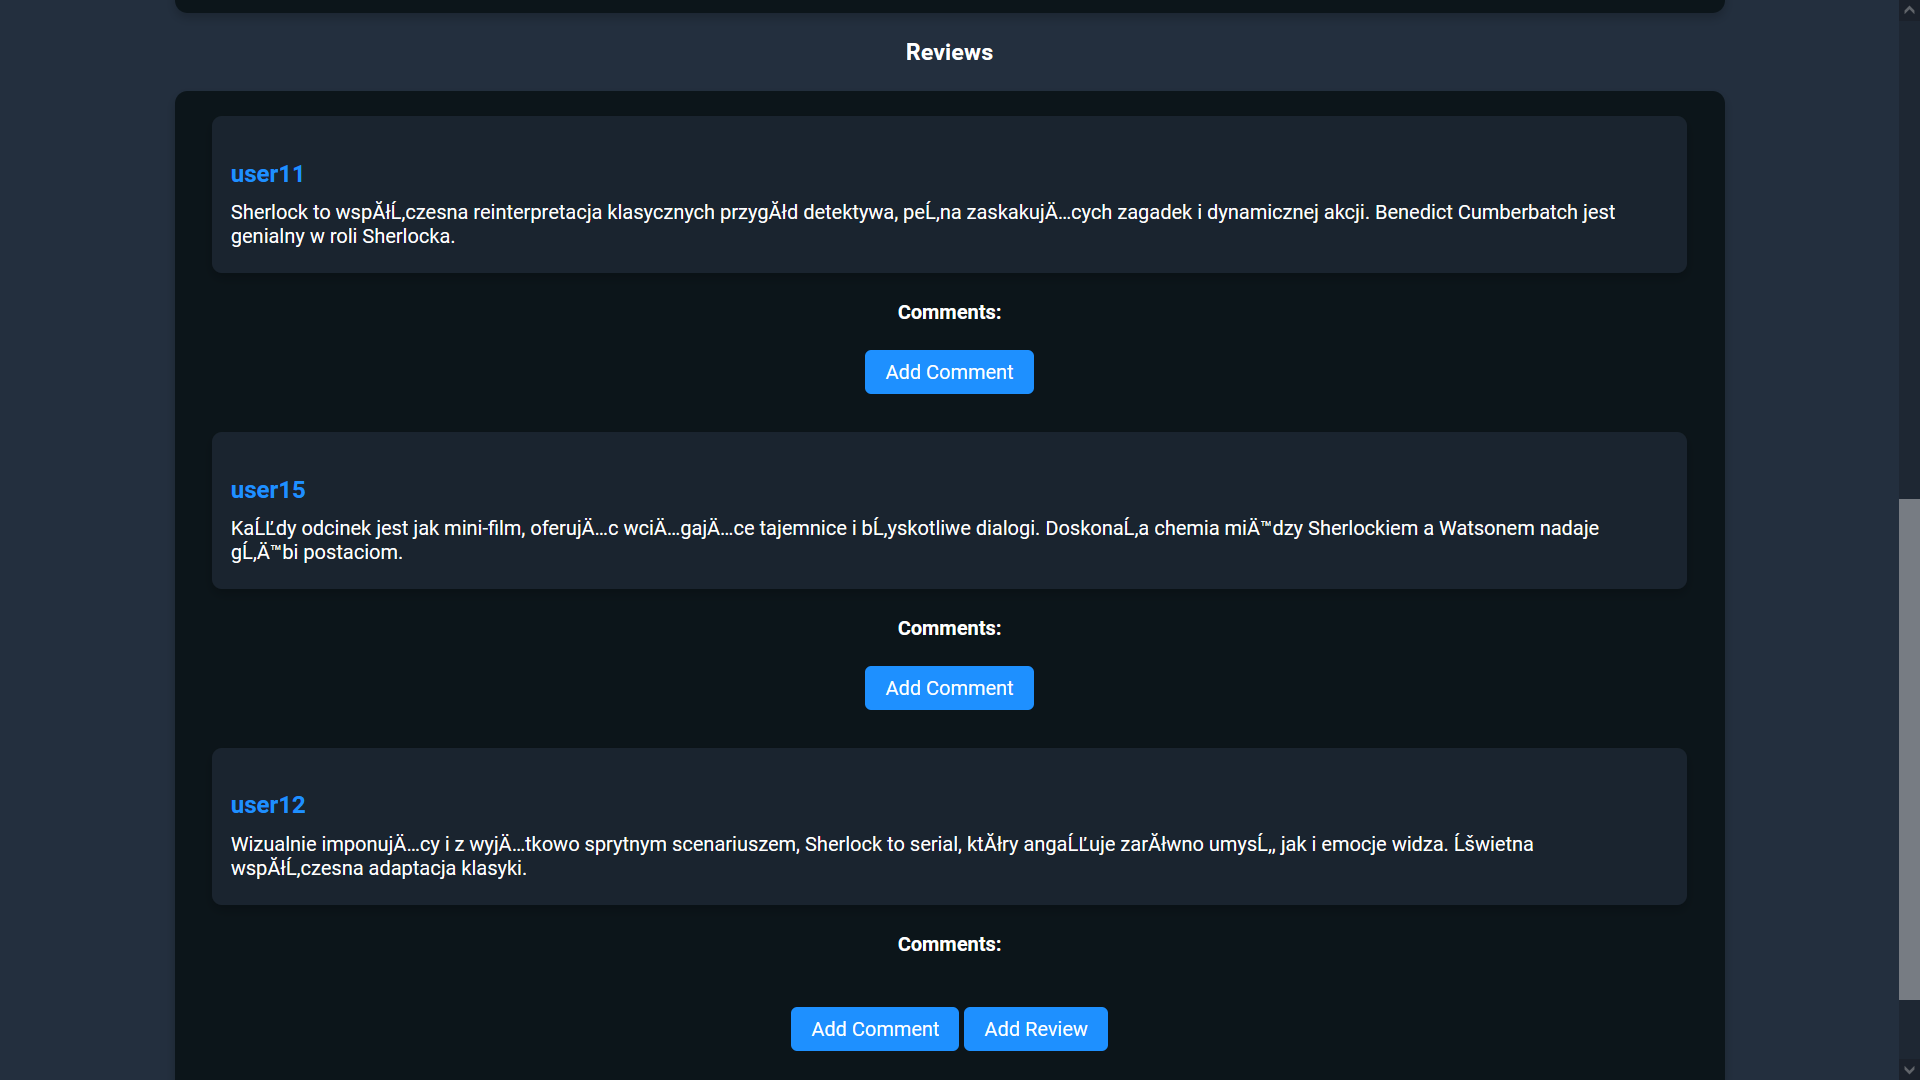
\includegraphics[width=\textwidth]{instrukcja_uzytkowania/movie_reviews.png}
	\caption{Widok filmu - recenzje}
	\label{fig:instrukcja_uzytkowania:movie_reviews}
\end{figure}

Następnie udostępniony jest użytkownikowi widok \textit{About}. Widok ten zawiera krótki opis aplikacji.

Ostatni widok dostępny z paska dla niezalogowanego użytkownika to widok \textit{Login} (rys. \ref{fig:instrukcja_uzytkowania:login}). Stamtąd użytkownik ma możliwość przejścia do widoku rejestracji (rys. \ref{fig:instrukcja_uzytkowania:register}), gdzie może założyć nowe konto.

\begin{figure}[htb]
	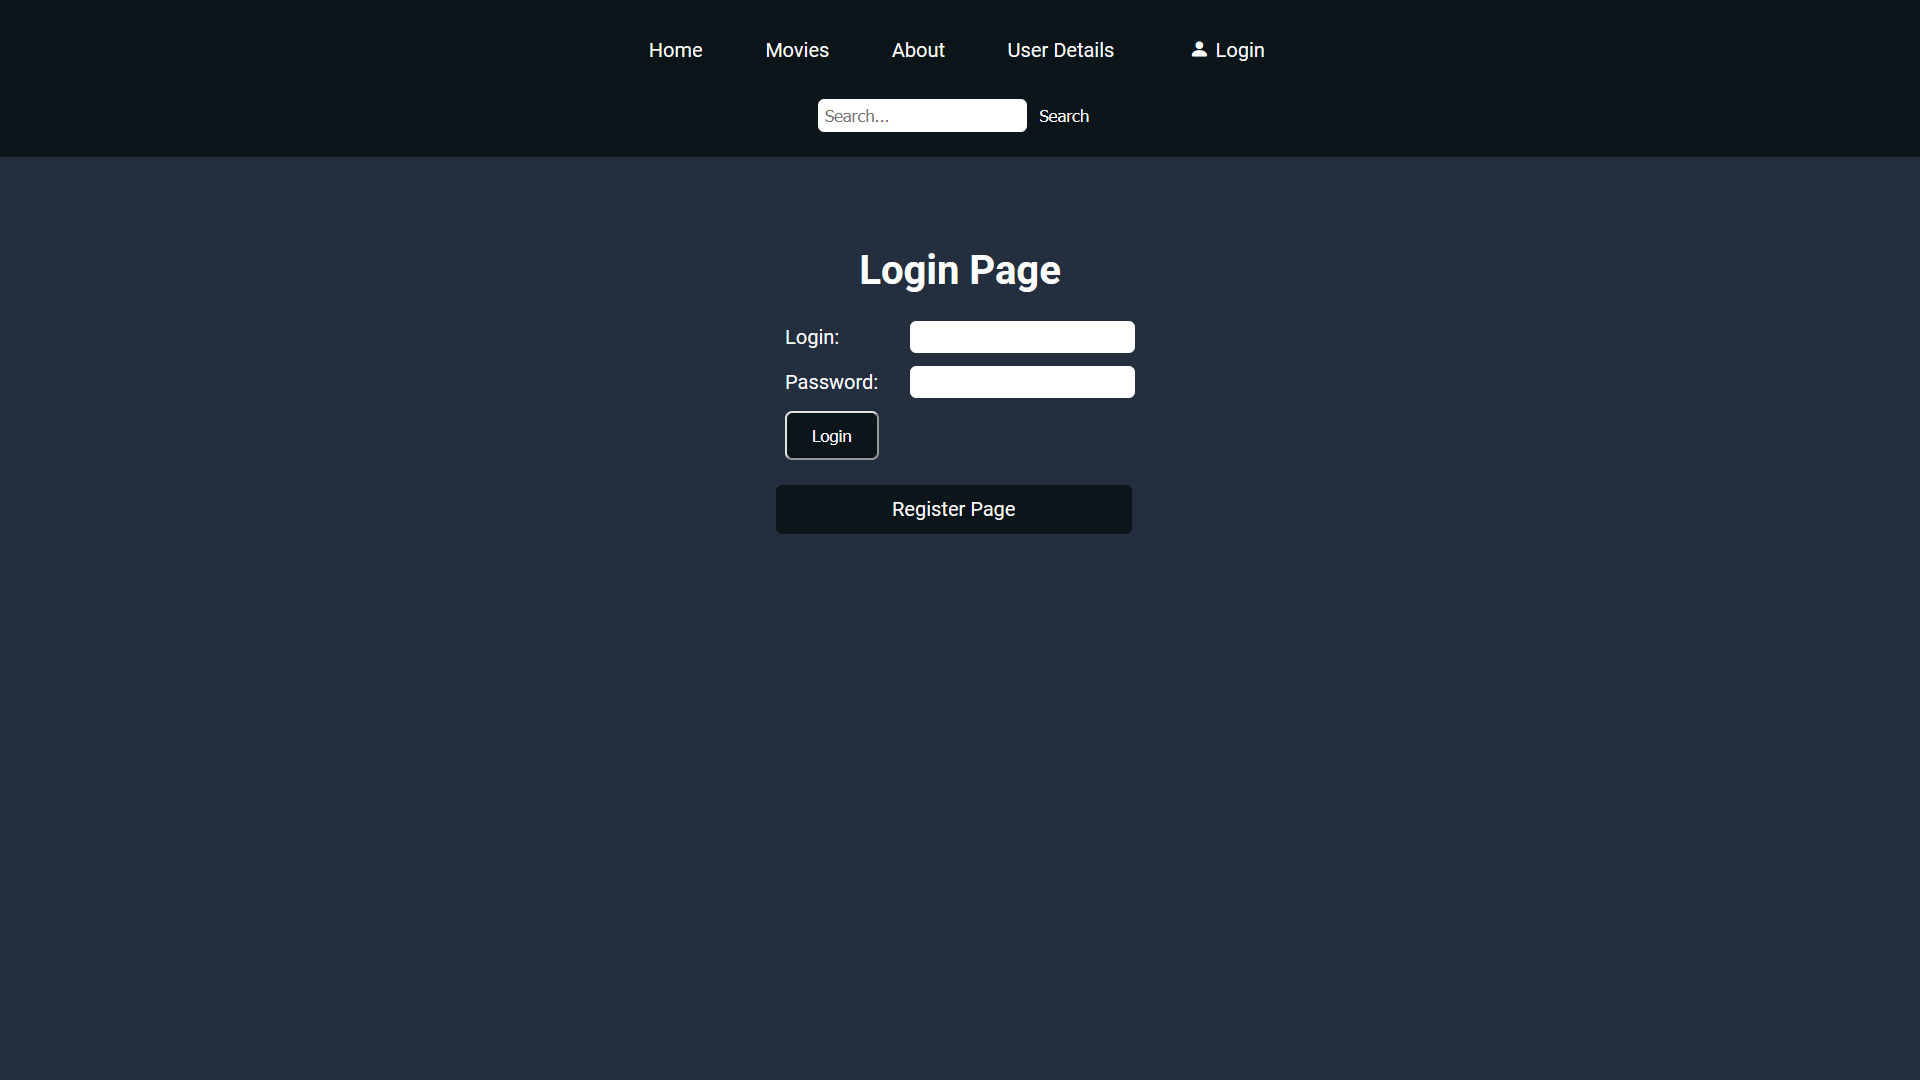
\includegraphics[width=\textwidth]{instrukcja_uzytkowania/login.png}
	\caption{Widok logowania}
	\label{fig:instrukcja_uzytkowania:login}
\end{figure}

\begin{figure}[htb]
	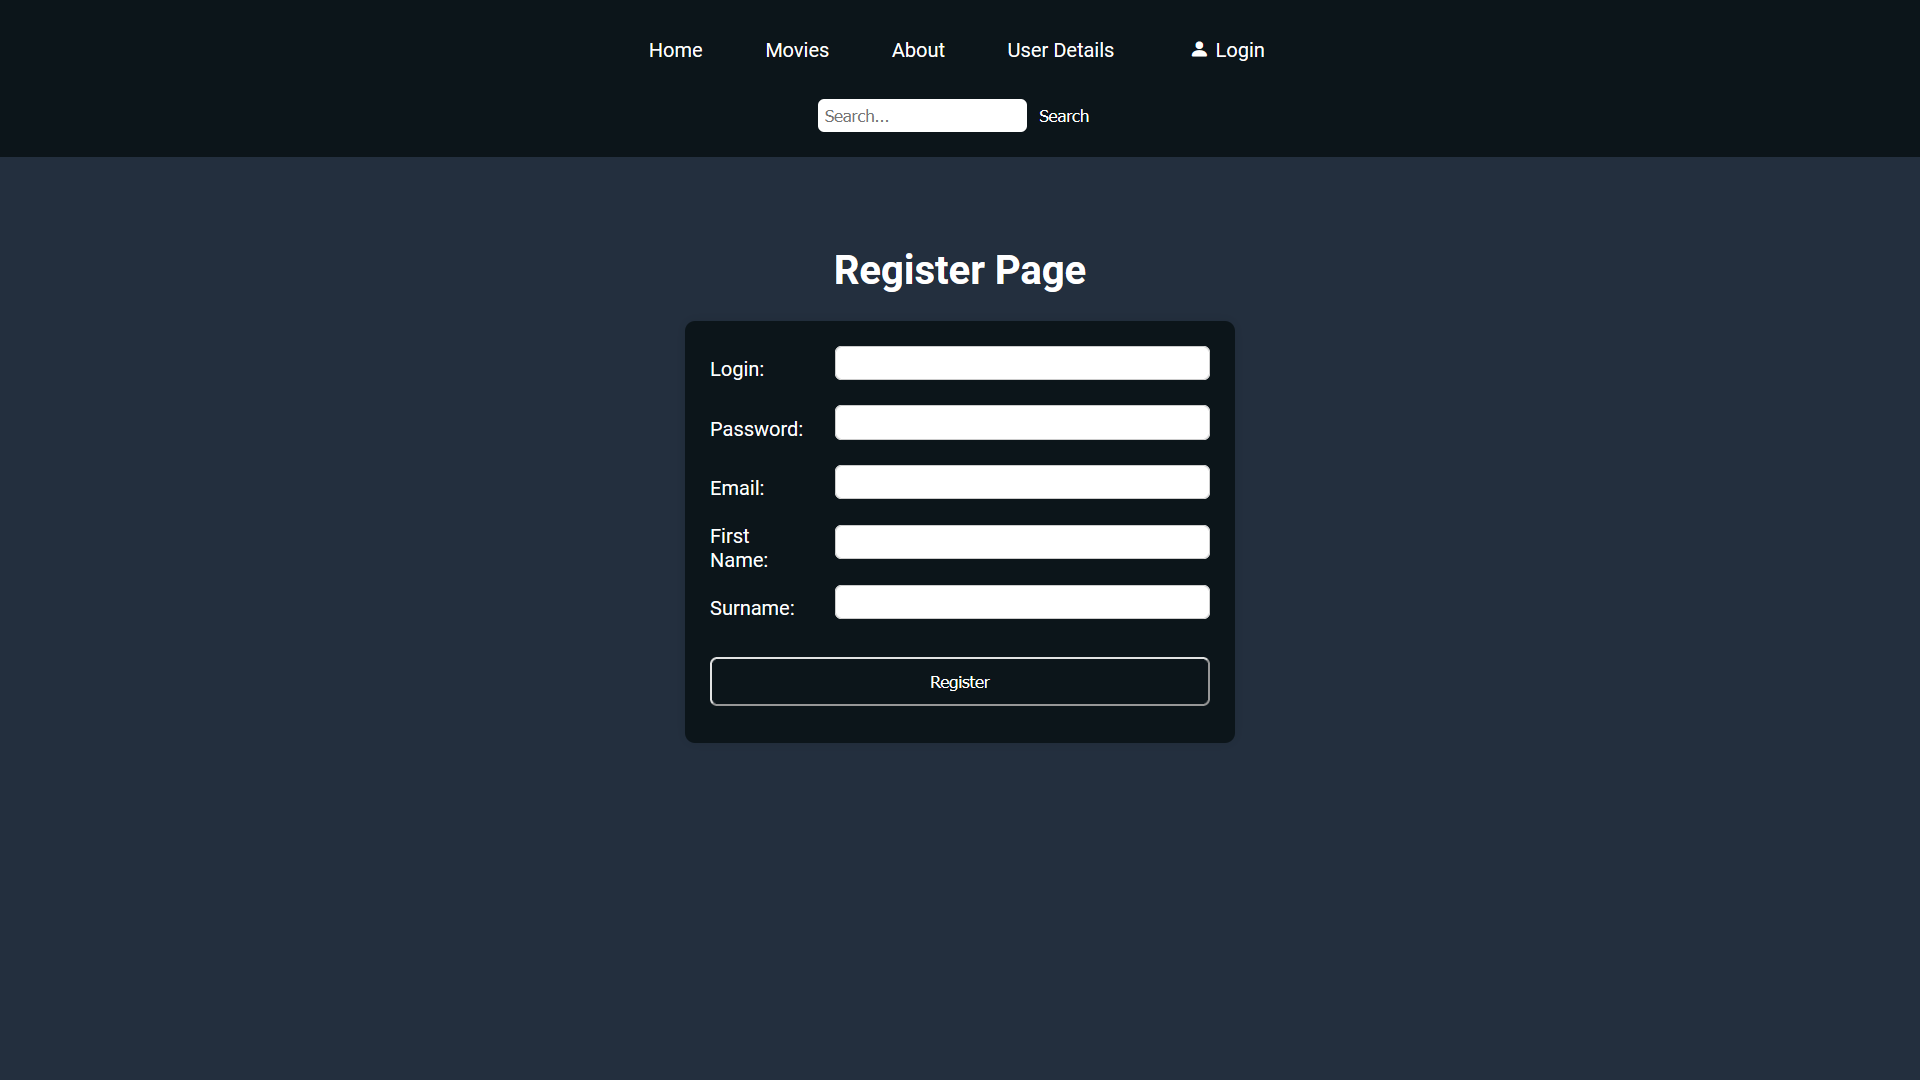
\includegraphics[width=\textwidth]{instrukcja_uzytkowania/register.png}
	\caption{Widok rejestracji}
	\label{fig:instrukcja_uzytkowania:register}
\end{figure}

Po zarejestrowaniu się i zalogowaniu, użytkownik ma dostęp do nowych funkcjonalności. Na karcie głównej (\textit{Home}), po wystawieniu co najmniej jednej pozytywnej recenzji filmu, pojawi się teraz sekcja rekomendacji (rys. \ref{fig:instrukcja_uzytkowania:recommended}). Znajdują się tam inteligentne rekomendacje, przygotowane specjalnie pod indywidualnego użytkownika.

\begin{figure}[htb]
	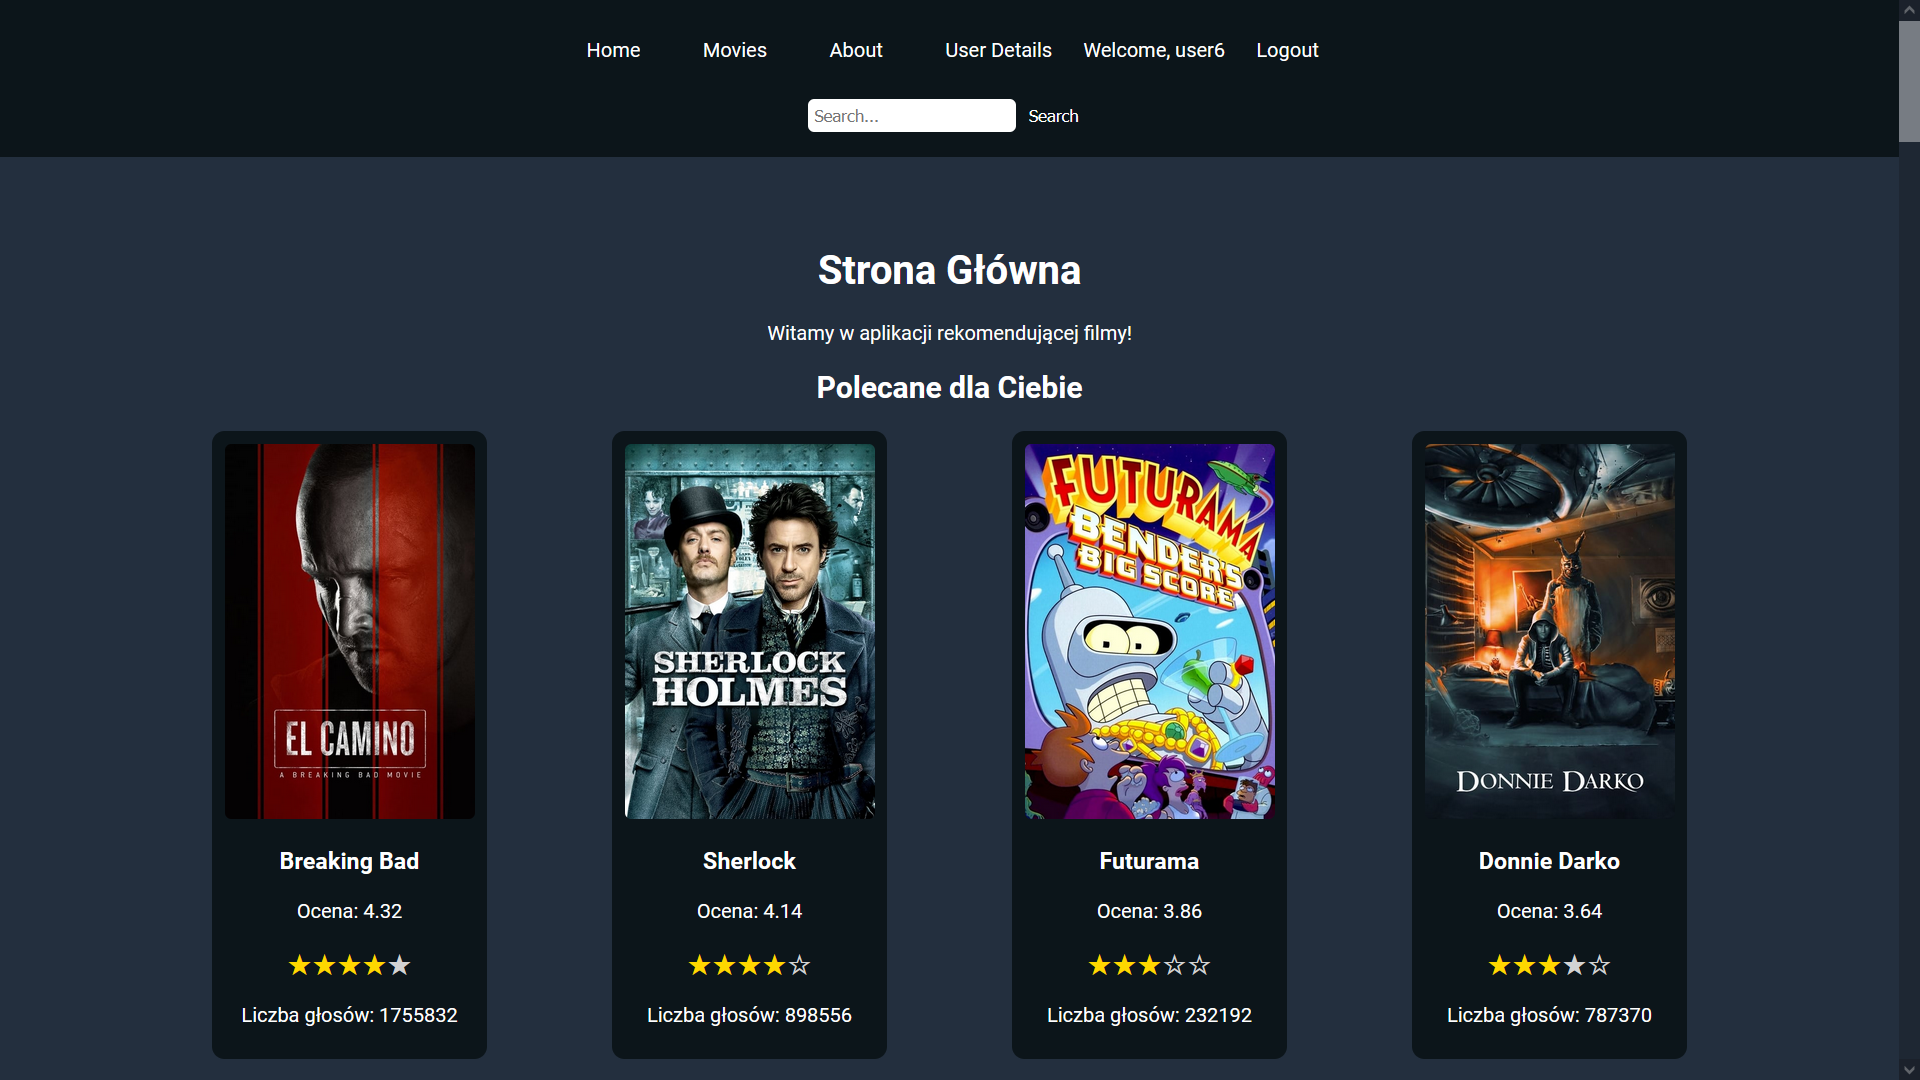
\includegraphics[width=\textwidth]{instrukcja_uzytkowania/recommended.png}
	\caption{Widok rekomendacji}
	\label{fig:instrukcja_uzytkowania:recommended}
\end{figure}

Następnie użytknownik ma możliwość wejścia w okno \textit{User details} (rys. \ref{fig:instrukcja_uzytkowania:user_details}). Znajdzie on tam informacje o swoim koncie oraz wystawione przez siebie recenzje (rys. \ref{fig:instrukcja_uzytkowania:reviews}).

\begin{figure}[htb]
	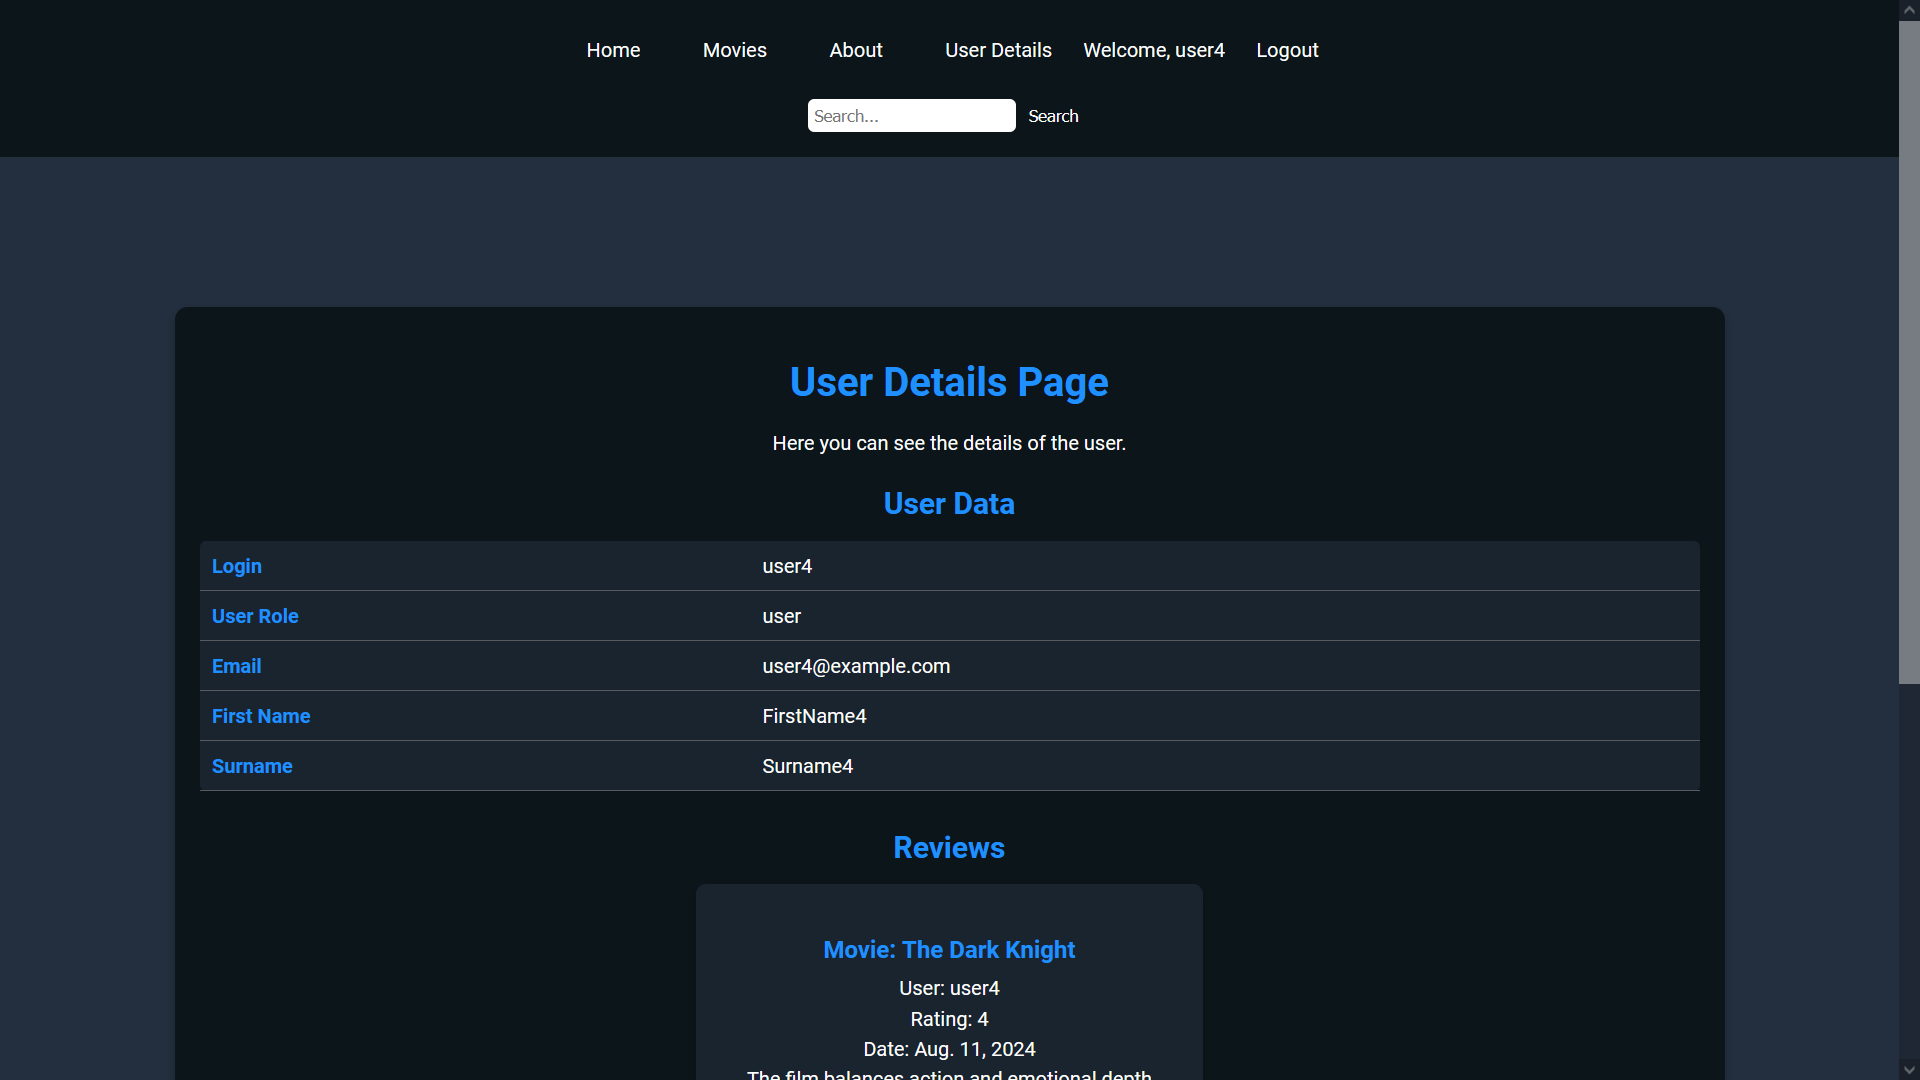
\includegraphics[width=\textwidth]{instrukcja_uzytkowania/user_details.png}
	\caption{Widok informacji o użytkowniku}
	\label{fig:instrukcja_uzytkowania:user_details}
\end{figure}

\begin{figure}[htb]
	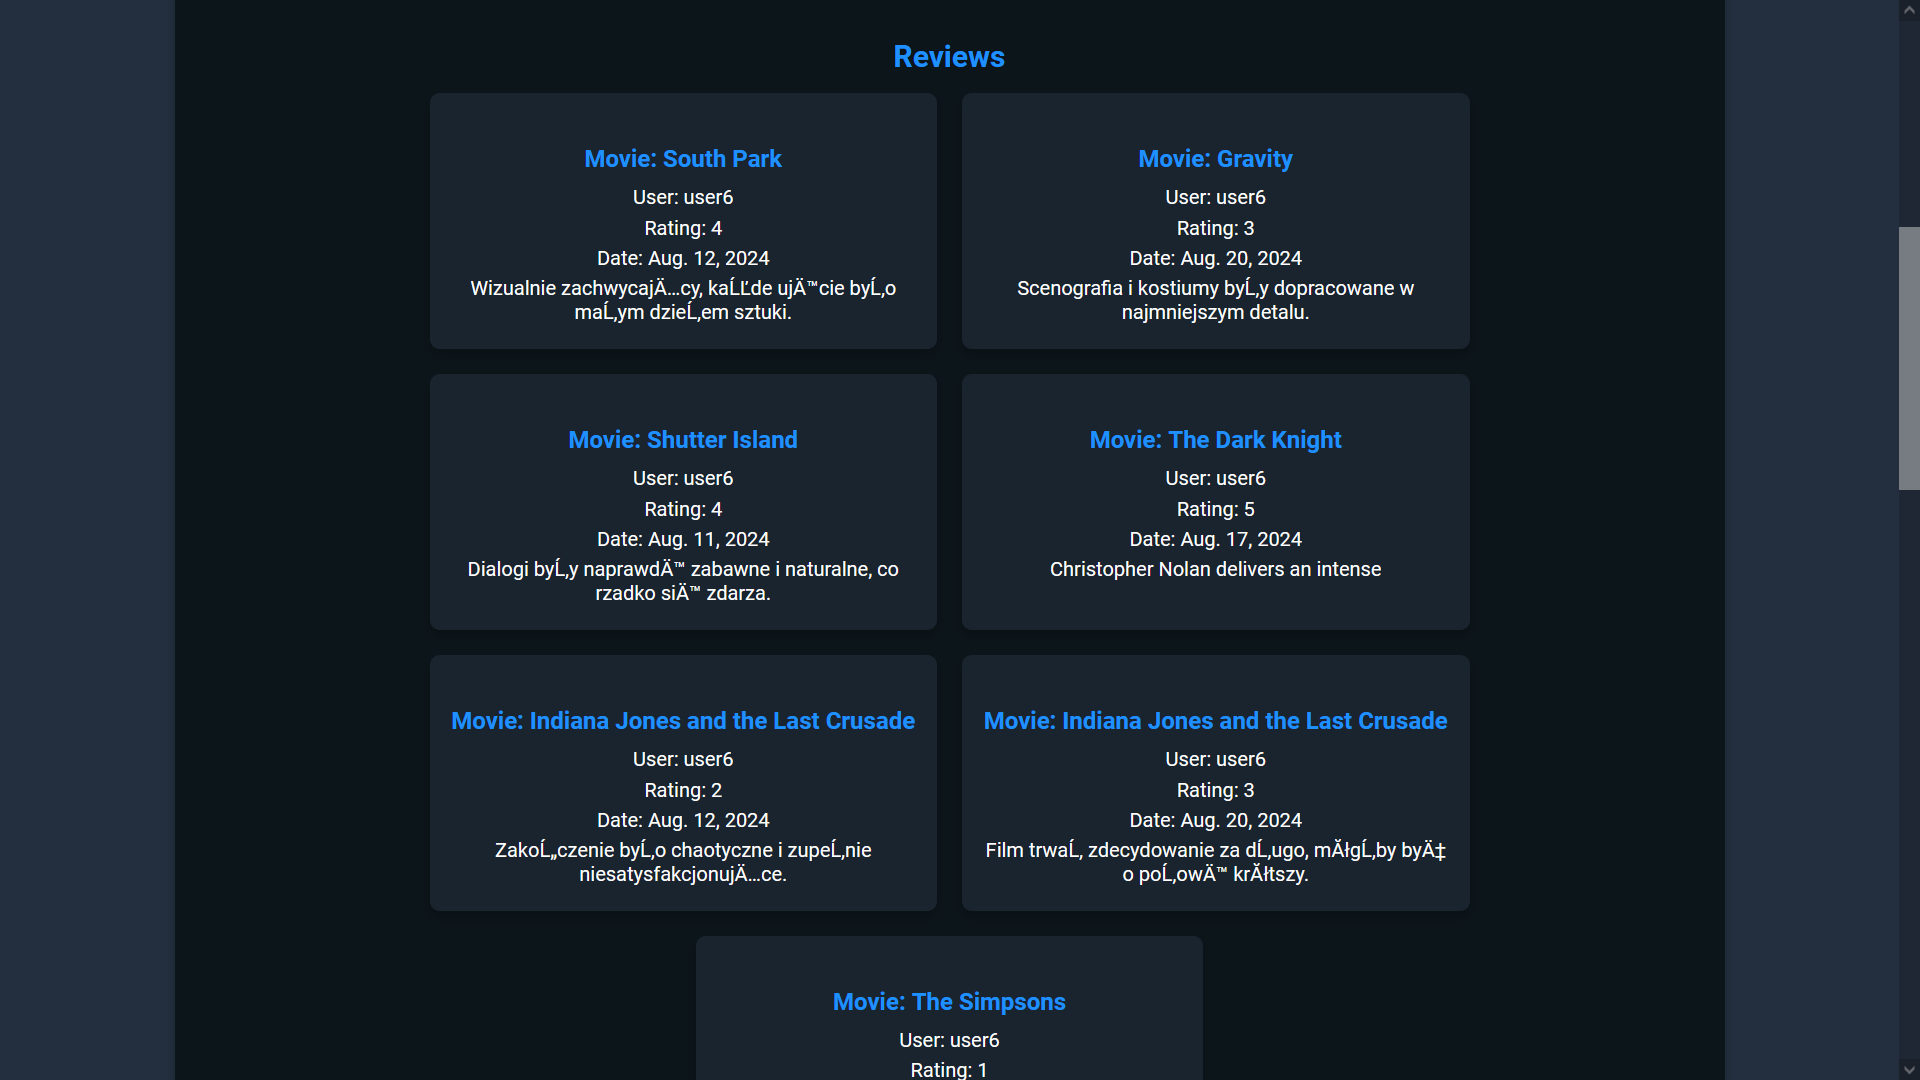
\includegraphics[width=\textwidth]{instrukcja_uzytkowania/reviews.png}
	\caption{Widok recenzji}
	\label{fig:instrukcja_uzytkowania:reviews}
\end{figure}


\end{document}